\section{Results}
\subsection{Forecast accuracy}
\begin{table*}[t]
\centering\small\setlength{\tabcolsep}{4pt}
\caption{Log-volatility RMSE. Lower is better. Each asset has 1,510 observations during 2019--2024 and 249 during 2025. The raw residual model has no ensemble shrinkage; the gated version uses the previous year's validation observations only.}
\label{tab:forecast}
\begin{tabular}{lrrrrrrrr}\toprule
&\multicolumn{4}{c}{2019--2024 exploratory}&\multicolumn{4}{c}{2025 confirmation}\\
\cmidrule(lr){2-5}\cmidrule(lr){6-9}
Forecast&SPY&IWM&TLT&GLD&SPY&IWM&TLT&GLD\\\midrule
Persistence & 0.0695 & 0.0603 & 0.0544 & 0.0655 & 0.0829 & 0.0677 & 0.0559 & 0.0775 \\
Window update & 0.0518 & 0.0440 & 0.0410 & 0.0491 & 0.0634 & 0.0472 & 0.0406 & 0.0608 \\
HAR-type OLS & 0.0683 & 0.0605 & 0.0542 & 0.0649 & 0.0805 & 0.0667 & 0.0559 & 0.0763 \\
EWMA & 0.1709 & 0.1312 & 0.1182 & 0.1210 & 0.2466 & 0.1465 & 0.0929 & 0.1687 \\
Level LSTM & 0.2004 & 0.2331 & 0.1468 & 0.0640 & 0.0652 & 0.0475 & 0.0421 & 0.0635 \\
Raw residual LSTM & 0.0569 & 0.0507 & 0.0448 & 0.0516 & 0.0641 & 0.0491 & 0.0400 & 0.0606 \\
Gated residual LSTM & 0.0573 & 0.0506 & 0.0448 & 0.0516 & 0.0641 & 0.0491 & 0.0400 & 0.0606
\\\bottomrule
\end{tabular}
\end{table*}
\begin{figure*}[t]
\centering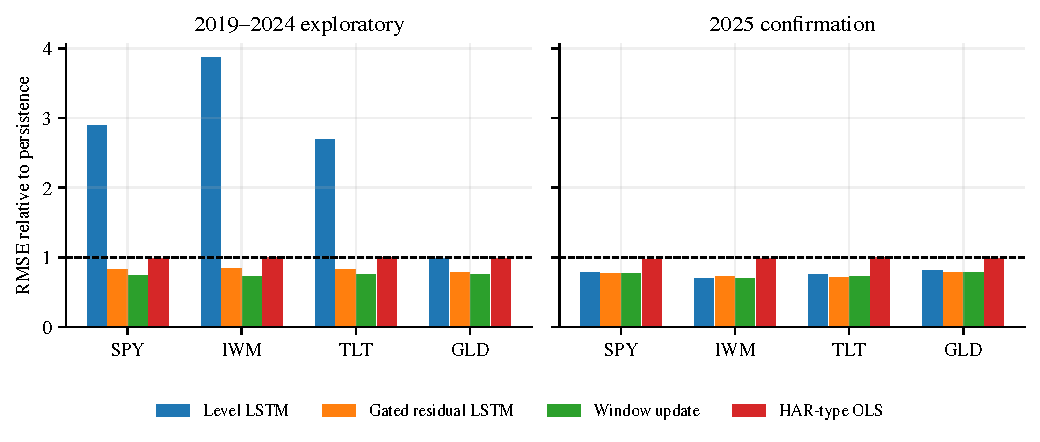
\includegraphics[width=\textwidth]{figures/study_forecast.pdf}
\caption{RMSE normalized by persistence, with the dashed line at one. Residual prediction removes much of the direct-level model's disadvantage. The window-update benchmark demonstrates that a substantial part of the gain concerns known rolling-window mechanics.}
\label{fig:forecast}
\end{figure*}

Table~\ref{tab:forecast} shows that the main neural comparison is materially different from a poorly performing level forecast. The gated residual model improves exploratory-period RMSE against persistence by 17.5\% for SPY, 16.0\% for IWM, 17.7\% for TLT, and 21.3\% for GLD. The corresponding confirmation improvements are approximately 22.6\%, 27.6\%, 28.5\%, and 21.8\%. Paired bootstrap intervals for residual-minus-persistence MSE lie below zero for all eight asset--period comparisons. These intervals are unadjusted descriptive summaries, not a claim of simultaneous or universal dominance.

The validation gate is one in 24 of the 28 asset--year fits and 0.75 in four. Thus the selected model does not achieve its result merely by reverting to persistence. The raw residual model is already substantially better than persistence; validation shrinkage makes relatively small changes. Reconstructing validation predictions from all saved residual checkpoints confirms that selected validation MSE never exceeds the persistence candidate's MSE.

The result is not evidence that neural complexity is essential. Equation~\eqref{eq:update} beats the selected residual model by RMSE for every asset in 2019--2024. Its residual-minus-update MSE intervals are positive. In 2025 the residual model is slightly better than the update forecast for TLT and GLD and slightly worse for SPY and IWM; all four corresponding difference intervals include zero. Figure~\ref{fig:forecast} therefore supports a narrower conclusion: an identity-anchored architecture is a fairer neural implementation, while simple conditional-moment structure remains highly competitive.

The level LSTM also performs considerably better in the confirmation year than in the exploratory aggregate, and its IWM RMSE is slightly lower than residual RMSE in 2025. This variation discourages a blanket claim that residual learning must outperform all level architectures. The main comparison includes EWMA, HAR-type OLS, and future five-day variation diagnostics in Appendix~\ref{app:forecast}, which distinguish predictability of the smoothed target from forecasting latent or forward risk.

\subsection{Calibration and predictive log scores}
\begin{table*}[t]
\centering\small
\caption{Parameters available at the start of 2025, estimated exclusively from past returns. $\theta$ is annual variance and $\mu$ annual physical drift. The final column is the standard deviation of total fitting log likelihood over five 4,096-particle evaluations; it is numerical variation, not a parameter standard error. Parameters are displayed to two significant figures.}
\label{tab:calibration}
\begin{tabular}{lrrrrrr}\toprule
ETF&$\kappa$&$\theta$&$\xi$&$\rho$&$\mu$&MC log-likelihood SD\\\midrule
SPY & 7.3 & 0.031 & 0.46 & -0.84 & 0.099 & 0.16 \\
IWM & 4.4 & 0.054 & 0.28 & -0.49 & 0.038 & 0.066 \\
TLT & 0.82 & 0.032 & 0.11 & -0.85 & -0.13 & 0.091 \\
GLD & 23 & 0.022 & 0.44 & 0.53 & 0.13 & 0.10
\\\bottomrule
\end{tabular}
\end{table*}
\begin{table*}[t]
\centering\small
\caption{Out-of-sample one-day return log scores from the latent-state filters. Higher is better. Difference is fitted minus the legacy fixed-parameter reference. Intervals are paired stationary-bootstrap summaries conditional on the fitted paths.}
\label{tab:logscores}
\begin{tabular}{llrrrr}\toprule
ETF&Period&Fitted&Fixed&Difference&95\% interval\\\midrule
SPY & 2019--24 & 3.2210 & 3.2256 & -0.0046 & [-0.0181, 0.0083] \\
SPY & 2025 & 3.2978 & 3.2803 & 0.0175 & [0.0007, 0.0360] \\
IWM & 2019--24 & 2.8120 & 2.8357 & -0.0237 & [-0.0469, -0.0050] \\
IWM & 2025 & 2.8924 & 2.9009 & -0.0085 & [-0.0250, 0.0075] \\
TLT & 2019--24 & 3.1533 & 3.1739 & -0.0206 & [-0.0832, 0.0173] \\
TLT & 2025 & 3.4925 & 3.4753 & 0.0172 & [-0.0005, 0.0352] \\
GLD & 2019--24 & 3.2730 & 3.2552 & 0.0179 & [-0.0181, 0.0444] \\
GLD & 2025 & 3.0122 & 2.9298 & 0.0824 & [0.0091, 0.1792]
\\\bottomrule
\end{tabular}
\end{table*}

Table~\ref{tab:calibration} reports asset-specific estimates available before 2025. Mean reversion ranges from about 0.82 for TLT to 23 for GLD, and return--variance correlation ranges from about $-0.85$ to $0.53$. Complete annual records appear in Appendix~\ref{app:parameters}. No retained fit lies within 1\% of a declared search boundary, but this does not establish parameter identification.

The fixed reference is a feasible candidate in the likelihood comparison. All 28 selected fitting scores exceed its score, so in-sample improvement is not an independent validation of the model. Out-of-sample results in Table~\ref{tab:logscores} are mixed: GLD has a higher mean fitted score in exploration, while SPY, IWM, and TLT have lower scores. In 2025 the fitted score is higher for SPY, TLT, and GLD and lower for IWM. The displayed confirmation intervals exclude zero for SPY and GLD, whereas those for TLT and IWM include zero. The exploratory IWM interval is below zero.

The reference uses common illustrative constants rather than a state-of-the-art likelihood estimator. All comparisons concern an approximate daily Euler model with bounded estimation and finite particles. They do not validate an exact continuous-time density or a market option surface.

\subsection{Fully invested portfolio outcomes}
\begin{table*}[t]
\centering\small\setlength{\tabcolsep}{4pt}
\caption{Broad model comparison with 2,000 scenarios at common unit gross ETF exposure. The higher-precision matched DRO comparison is in Table~\ref{tab:paired}. CAGR, daily loss ES, and maximum drawdown (MDD, positive magnitude) are percentages. SR is excess-return Sharpe against 3\% cash and $N_{\rm eff}$ the average effective ETF count. Calendar slices contain 1,508 and 247 daily returns. Holdings are carried into 2025 rather than restarted.}
\label{tab:portfolio}
\begin{tabular}{lrrrrrrrrrr}\toprule
&\multicolumn{5}{c}{2019--2024 exploratory}&\multicolumn{5}{c}{2025 confirmation}\\
\cmidrule(lr){2-6}\cmidrule(lr){7-11}
Strategy&CAGR&SR&ES&MDD&$N_{\rm eff}$&CAGR&SR&ES&MDD&$N_{\rm eff}$\\\midrule
Buy and hold & 10.36 & 0.627 & 1.83 & 25.16 & 3.85 & 31.57 & 1.946 & 1.95 & 11.32 & 3.50 \\
Equal weight & 9.98 & 0.605 & 1.77 & 24.65 & 4.00 & 26.80 & 1.796 & 1.72 & 10.49 & 4.00 \\
Minimum variance & 8.02 & 0.509 & 1.49 & 24.91 & 2.88 & 42.98 & 3.045 & 1.52 & 5.08 & 2.55 \\
Historical mean--CVaR & 4.36 & 0.164 & 2.20 & 32.77 & 1.78 & 61.25 & 2.675 & 2.53 & 8.24 & 1.21 \\
Fitted Heston / filter & 11.26 & 0.790 & 1.59 & 23.72 & 2.49 & 49.91 & 3.014 & 1.87 & 5.60 & 1.85 \\
Fitted Heston / persistence & 11.17 & 0.776 & 1.61 & 22.21 & 2.37 & 45.62 & 2.890 & 1.90 & 5.62 & 1.88 \\
Fitted Heston / residual & 11.04 & 0.766 & 1.60 & 22.55 & 2.37 & 45.83 & 2.926 & 1.87 & 5.62 & 1.88 \\
Fixed parameters / residual & 11.57 & 0.801 & 1.65 & 22.62 & 2.28 & 41.72 & 2.740 & 1.81 & 6.11 & 1.89 \\
Gaussian / residual & 11.62 & 0.796 & 1.67 & 22.21 & 2.20 & 41.28 & 2.710 & 1.82 & 6.00 & 1.85 \\
Fixed-radius DRO & 11.08 & 0.770 & 1.60 & 22.49 & 2.40 & 46.02 & 2.936 & 1.87 & 5.64 & 1.90 \\
Adaptive-radius DRO & 11.02 & 0.766 & 1.60 & 22.54 & 2.44 & 46.45 & 2.971 & 1.85 & 5.68 & 1.93
\\\bottomrule
\end{tabular}
\end{table*}
\begin{figure*}[t]
\centering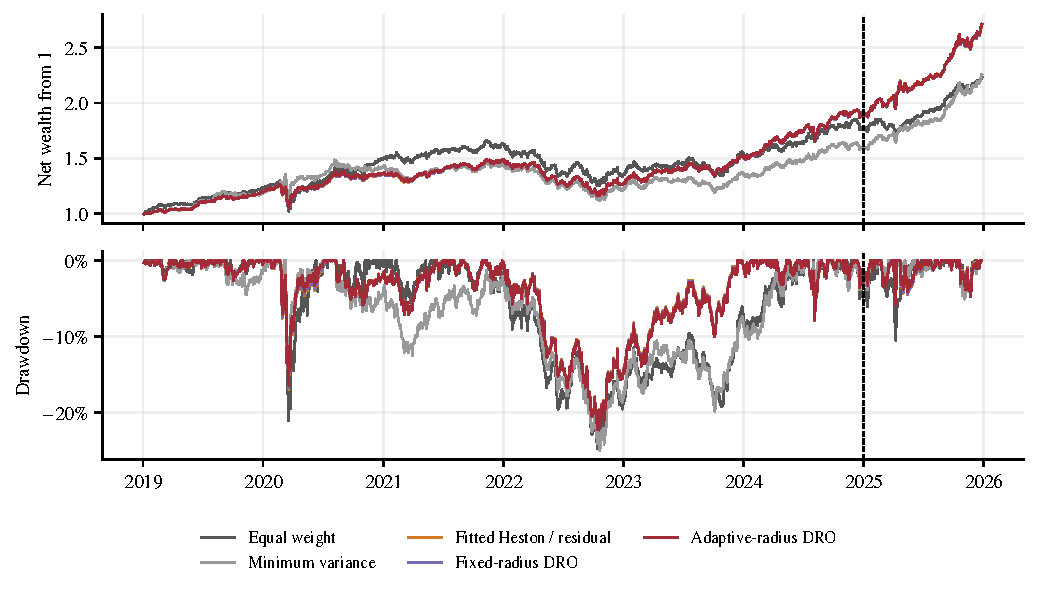
\includegraphics[width=\textwidth]{figures/study_wealth.pdf}
\caption{Net wealth and daily drawdown at equal total ETF exposure. Nominal and DRO curves use the primary 20,000-scenario seed; equal weight and minimum variance are historical-input references. The vertical line separates the exploratory sample from 2025 confirmation. A single favorable confirmation year does not establish persistent investment superiority.}
\label{fig:wealth}
\end{figure*}

The broad model comparison (Table~\ref{tab:portfolio}) is complemented by a matched higher-scenario experiment. The main economic assessment of robustness uses 20,000 scenarios and three independent seeds. All model parameters, expected returns, costs, and preferences are held common within that comparison; only the ambiguity radius differs. Holdings carry through the full historical path for each strategy and seed.

\begin{table*}[t]
\centering\small\setlength{\tabcolsep}{4pt}
\caption{Primary matched comparison at 20,000 scenarios, seed offset zero. Units match Table~\ref{tab:portfolio}; other seed outcomes are in Appendix~\ref{app:sensitivity}. The first seed was fixed in advance of this numerical comparison and was not chosen for its return.}
\label{tab:paired}
\begin{tabular}{lrrrrrrrrrr}\toprule
&\multicolumn{5}{c}{2019--2024 exploratory}&\multicolumn{5}{c}{2025 confirmation}\\
\cmidrule(lr){2-6}\cmidrule(lr){7-11}
Strategy&CAGR&SR&ES&MDD&$N_{\rm eff}$&CAGR&SR&ES&MDD&$N_{\rm eff}$\\\midrule
Fitted Heston / residual & 11.20 & 0.779 & 1.61 & 22.11 & 2.38 & 44.06 & 2.792 & 1.91 & 5.69 & 1.90 \\
Fixed-radius DRO & 11.18 & 0.779 & 1.60 & 22.19 & 2.42 & 44.39 & 2.810 & 1.91 & 5.74 & 1.92 \\
Adaptive-radius DRO & 11.21 & 0.783 & 1.60 & 22.25 & 2.46 & 44.59 & 2.849 & 1.88 & 5.82 & 1.95
\\\bottomrule
\end{tabular}
\end{table*}

In the primary 20,000-scenario path, nominal residual Heston earns 11.20\% exploratory CAGR and adaptive DRO 11.21\%. Their daily loss ES values are 1.606\% and 1.598\%. Adaptive DRO's maximum drawdown is 22.25\%, compared with 22.11\% nominally: smaller ES does not mean every realized risk measure improves. The corresponding confirmation CAGRs are 44.06\% and 44.59\%, with ES of 1.911\% and 1.881\%.

Every matched nominal and DRO rebalance in all three seeds holds at least two ETFs above the reporting threshold. Primary adaptive-DRO effective counts average 2.46 during exploration and 1.95 during confirmation, compared with nominal counts of 2.38 and 1.90. No per-asset cap forces these mixtures. Figure~\ref{fig:weights} shows primary-seed weights.

The 2,000-scenario model comparisons describe different scenario specifications rather than determine the main DRO conclusion. Filter-initialized Heston earns 49.91\% confirmation CAGR; historical mean--CVaR earns 61.25\% with greater concentration and tail loss. GLD's 63.7\% calendar return and the historical strategy's mean GLD weight of 90.2\% explain why that latter result is effectively a gold bet. The effective asset count is only 1.21. This is a favorable regime for concentrated gold exposure, not general confirmation of predictive superiority.

Fixed-parameter and Gaussian ablations slightly outperform the fitted residual specification by exploratory CAGR but trail it in confirmation. Estimation and stochastic-volatility dynamics are modeling choices whose economic value remains empirical. The residual forecast's incremental portfolio effect relative to persistence is also small. The broad 2,000-scenario and primary 20,000-scenario CAGRs differ because empirical tail approximations affect the optimizer; their difference motivates the matched higher-scenario comparison rather than a selection of the more favorable run.

\begin{figure*}[t]
\centering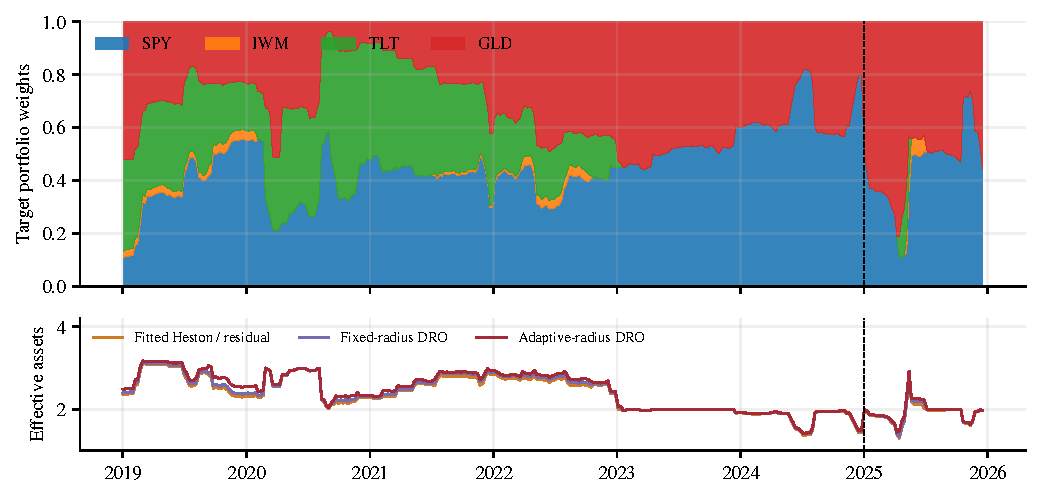
\includegraphics[width=\textwidth]{figures/study_weights.pdf}
\caption{Primary 20,000-scenario adaptive-DRO weights and effective ETF counts of matched model variants. Total ETF weight is one throughout. Allocations vary over time and hold multiple assets; the primary experiment cannot explain gains through an all-cash position.}
\label{fig:weights}
\end{figure*}

\subsection{Uncertainty, cash, and numerical scale}
\begin{table*}[t]
\centering\small\setlength{\tabcolsep}{4pt}
\caption{Robust allocation minus matched nominal residual Heston, at 20,000 scenarios and primary seed zero. Mean-return differences are annualized arithmetic percentage points. Daily ES differences are basis points, with negative values indicating lower tail loss. Intervals are unadjusted paired bootstrap percentiles.}
\label{tab:bootstrap}
\begin{tabular}{llrrrr}\toprule
Period&Robust strategy&Mean diff.&95\% interval&ES diff.&95\% interval\\\midrule
2019--24 & Fixed-radius DRO & -0.02 & [-0.11, 0.10] & -0.33 & [-0.81, 0.02] \\
2019--24 & Adaptive-radius DRO & 0.00 & [-0.23, 0.31] & -0.81 & [-2.04, 0.04] \\
2025 & Fixed-radius DRO & 0.23 & [-0.30, 0.82] & -0.03 & [-2.07, 2.45] \\
2025 & Adaptive-radius DRO & 0.35 & [-0.72, 1.46] & -3.02 & [-11.44, 4.14]
\\\bottomrule
\end{tabular}
\end{table*}
\begin{table*}[t]
\centering\small
\caption{Cash-enabled secondary experiment with 2,000 scenarios. CAGR and daily ES are percentages. Gross is mean risky ETF exposure in percent. The remaining wealth earns stylized 3\% annual cash interest. These portfolios solve a different mandate from the fully invested primary experiment.}
\label{tab:cash}
\begin{tabular}{lrrrrrr}\toprule
&\multicolumn{3}{c}{2019--2024 exploratory}&\multicolumn{3}{c}{2025 confirmation}\\
\cmidrule(lr){2-4}\cmidrule(lr){5-7}
Strategy&CAGR&ES&Gross&CAGR&ES&Gross\\\midrule
Fitted Heston / persistence & -0.03 & 1.20 & 38.75 & 5.49 & 0.13 & 3.82 \\
Fitted Heston / residual & -0.21 & 1.18 & 38.42 & 4.70 & 0.05 & 1.88 \\
Fixed-radius DRO & -0.48 & 1.16 & 37.03 & 3.71 & -0.01 & 0.35 \\
Adaptive-radius DRO & -0.54 & 1.12 & 35.19 & 3.16 & -0.01 & 0.08
\\\bottomrule
\end{tabular}
\end{table*}

Table~\ref{tab:bootstrap} shows no statistically reliable return advantage for either robust rule over matched nominal allocation. For adaptive DRO, the exploratory annualized arithmetic mean-return difference is approximately 0.003 percentage points, with interval $[-0.23,0.31]$. In confirmation the difference is 0.35 points, with interval $[-0.72,1.46]$. The primary-seed ES-difference intervals also include zero. These are descriptive, unadjusted intervals conditional on fitted paths.

The other two seeds preserve the direction of the confirmation return difference but do not establish significance. Across seeds, adaptive-minus-nominal mean-return differences range from about 0.08 to 0.35 annual percentage points in 2025; every corresponding interval includes zero. ES point differences are negative in both periods under all seeds. Two exploratory ES intervals exclude zero, whereas the primary interval and all confirmation intervals include zero. We do not select a seed because its interval is more favorable.

The conditional allocation experiment separates this statistical uncertainty from numerical resolution. At 2,000 scenarios, independent-seed adaptive-weight distances average about 0.022, exceeding within-seed robustness tilts of about 0.011--0.012. At 20,000 scenarios, average distances fall to 0.0053--0.0059, below tilts of 0.0128--0.0134 (Appendix~\ref{app:sensitivity}). The 95th-percentile distances remain larger than the mean tilt, so some dates remain more sensitive than average. Higher-scenario sampling resolves a small average allocation effect without supplying evidence of a reliable return improvement.

Cash-enabled results (Table~\ref{tab:cash}) concern a different mandate. Mean exploratory risky exposure is about 38.4\% for residual Heston and 35.2\% for adaptive DRO, with negative CAGRs despite smaller daily ES. In confirmation those risky exposures are about 1.88\% and 0.08\%, respectively. Lower risk largely reflects cash holdings. Negative displayed loss ES is possible when even the average worst-tail daily return is positive in a mostly cash portfolio.

Reference quantiles are imperfect. In the 2,000-scenario experiment, nominal residual-Heston and adaptive-DRO portfolios each breach their reference 5\% return quantile in 23 of 302 exploratory holding intervals (7.62\%) and one of 49 confirmation intervals (2.04\%). A robust objective adjustment does not produce a predictive VaR quantile or guarantee ambiguity-set membership. Radius, quadratic-risk, and fee sensitivities are descriptive grids reported in the appendix; no value is selected by confirmation performance.
